\documentclass[
size=17pt,
paper=smartboard,
mode=present,
display=slidesnotes,
style=sailor,
nopagebreaks,
blackslide,
fleqn]{powerdot}
 %wj capsules prettybox
 %mode = handout or present

\usepackage{amsmath,graphicx,color,amsfonts}
\usepackage[brazilian]{babel}
\usepackage[utf8]{inputenc}

\pdsetup{
   lf = {EC01045 PDS},
   rf = {Sinais e Sistemas Discretos},palette = {Sea},randomdots={false}
}
% palette = {green}, 

%opening
\title{\Large EC01045 -- Processamento Digital de Sinais\\ \vspace{1cm}Sinais e Sistemas Discretos}
\author{Ronaldo de Freitas Zampolo\\FCT-ITEC-UFPA}
\date{ }


\begin{document}

   \maketitle[randomdots={false}]
   \begin{slide}{Agenda}
      \tableofcontents[content=sections]
   \end{slide}

\section[slide=false]{Sinais discretos}
   \begin{slide}[toc=]{Representação e amostragem}
      \begin{itemize}
         \item Representação:
         \begin{itemize}
            \item Sequência de números: $x$
            \item $n$-ésimo número da sequência: $x[n]$, $n \in \mathbb{Z}$
            \item $x=\{x[n]\},\quad -\infty < n < \infty$
         \end{itemize}
         \begin{itemize}
         \item Amostragem:
            \item $x[n]=x_a(nT), \quad -\infty < n < \infty$
            \item $T$: período de amostragem
            \item $f_s=1/T$: frequência de amostragem
         \end{itemize}
      \end{itemize}
   \end{slide}

\begin{slide}[toc=]{Representação gráfica}
   \begin{center}
     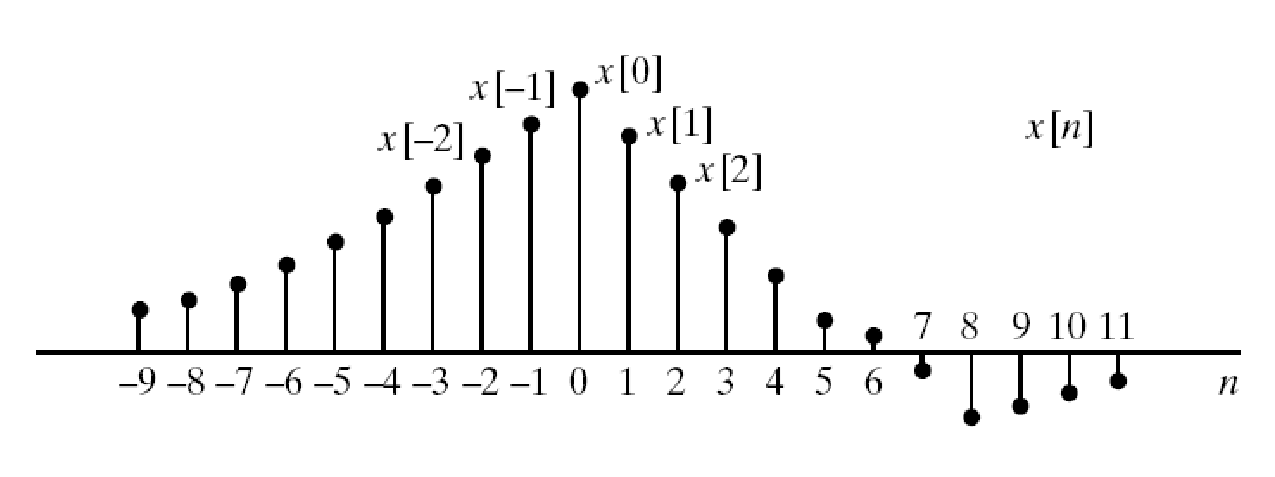
\includegraphics[width=\textwidth]{figs/2_1.eps}
   \end{center}
\end{slide}

\begin{slide}[toc=]{Amostragem de sinais contínuos}
\begin{itemize}
 \item Período de amostragem $T=125 \mu \text{s}$\\
    \begin{center}
       \onslide*{1}{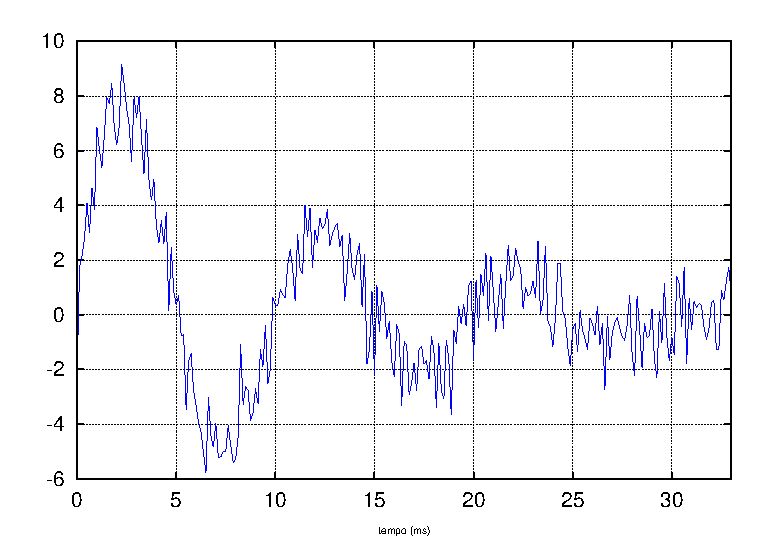
\includegraphics[width=0.7\textwidth]{figs/sCont.eps}}
      \onslide*{2}{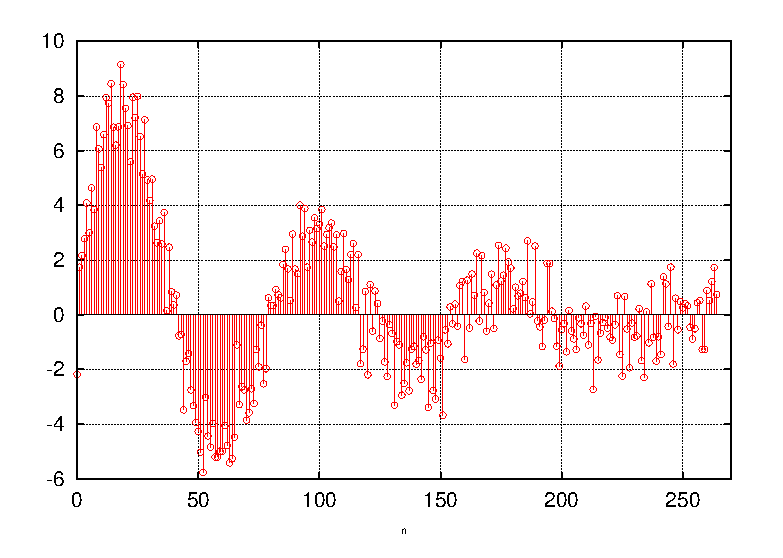
\includegraphics[width=0.7\textwidth]{figs/sDiscr.eps}}
      \onslide*{3}{$[ \begin{array}{ c c c c } -2,1738 &  1,7422 &  2,1658 &  \cdots \end{array} ]$}
    \end{center}
\end{itemize}
\end{slide}

\begin{slide}[toc=]{Operações básicas}
 \begin{itemize}
    \item
    \onslide*{1}{Sinais $x_1[n]$ e $x_2[n]$ \\
		 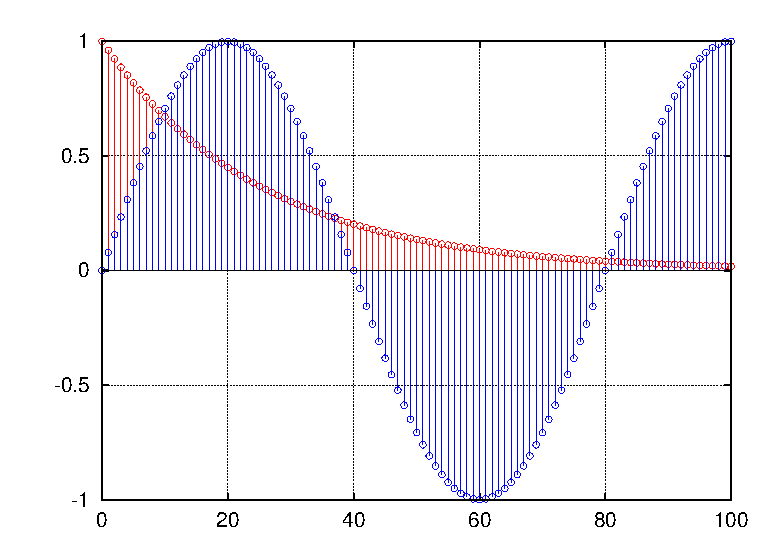
\includegraphics[width=0.7\textwidth]{figs/sX1eX2.eps}}
    \onslide*{2}{Soma de sinais: $x_1[n]+x_2[n]$
                          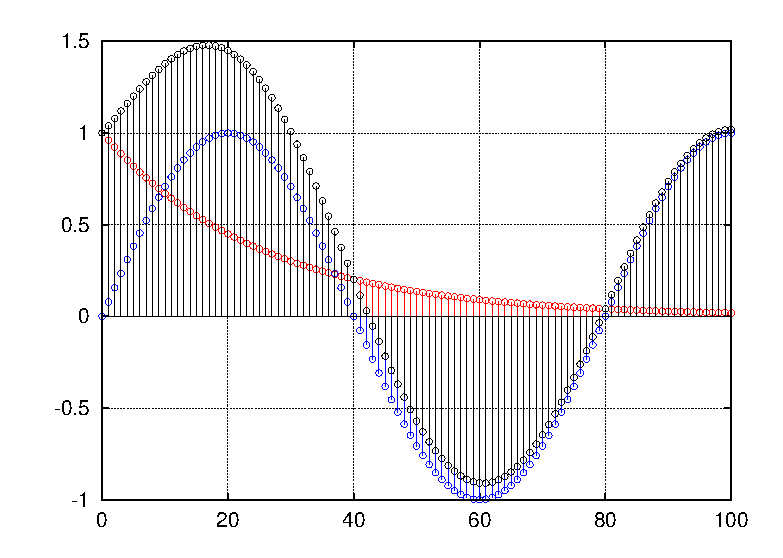
\includegraphics[width=0.7\textwidth]{figs/sX1maisX2.eps}} 
    \onslide*{3}{Multiplicação de sinais: $x_1[n]x_2[n]$
                          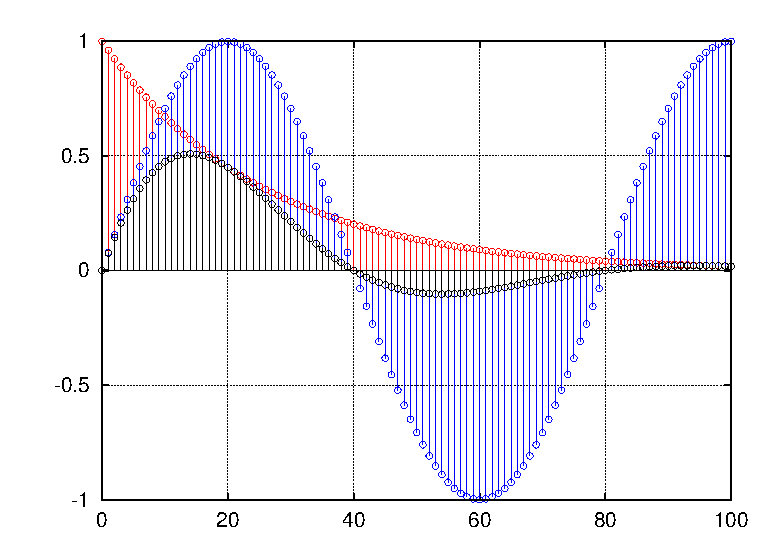
\includegraphics[width=0.7\textwidth]{figs/sX1vezesX2.eps} }
    \onslide*{4}{Multiplicação por escalar: $\alpha x[n]$ ($\alpha = 2$ e $0,5$)
                          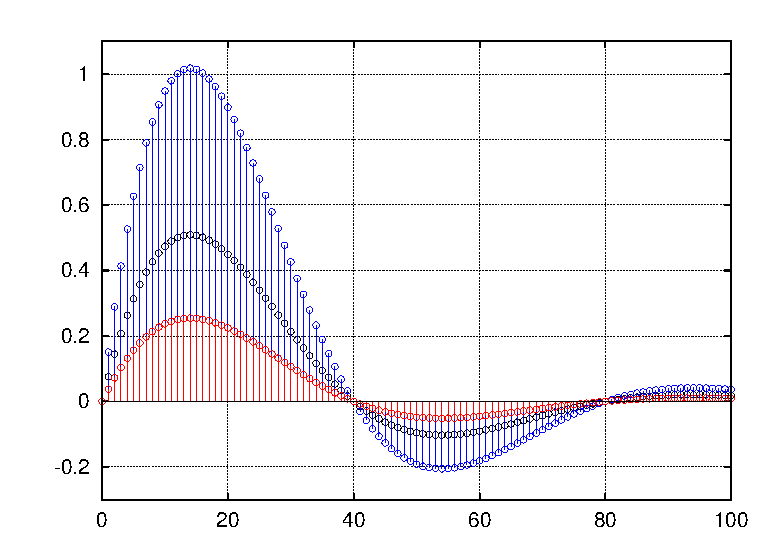
\includegraphics[width=0.7\textwidth]{figs/multConst.eps} }
    \onslide*{5}{Deslocamento: $x[n-n_o]$ ($n_o=20$)
                          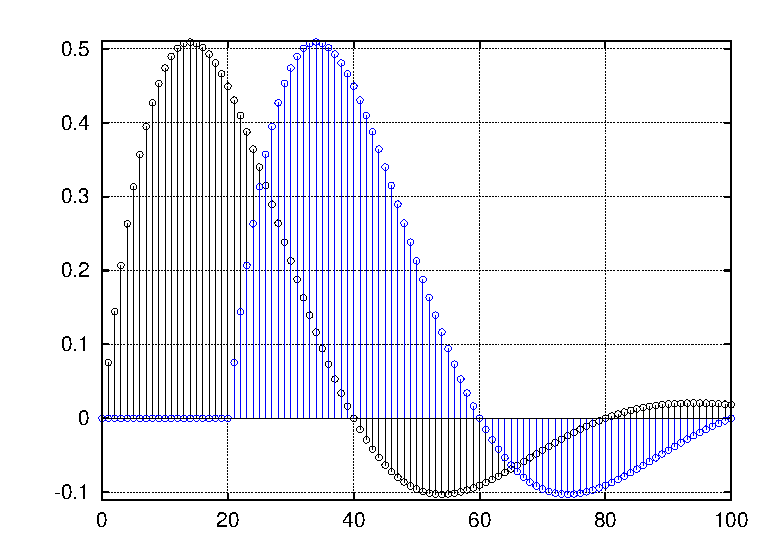
\includegraphics[width=0.7\textwidth]{figs/desloc.eps} }
  \end{itemize}
\end{slide}


\begin{slide}[toc=]{Sequências básicas 1}
\begin{itemize}
   \item Impulso unitário: 
      \onslide*{1-2}{
      \begin{equation*}
         \delta [n]=\begin{cases}
                  0, & n\neq 0,\\
                  1, & n=0,
                 \end{cases}
       \end{equation*}}
      \onslide*{2}{
      \begin{center}
        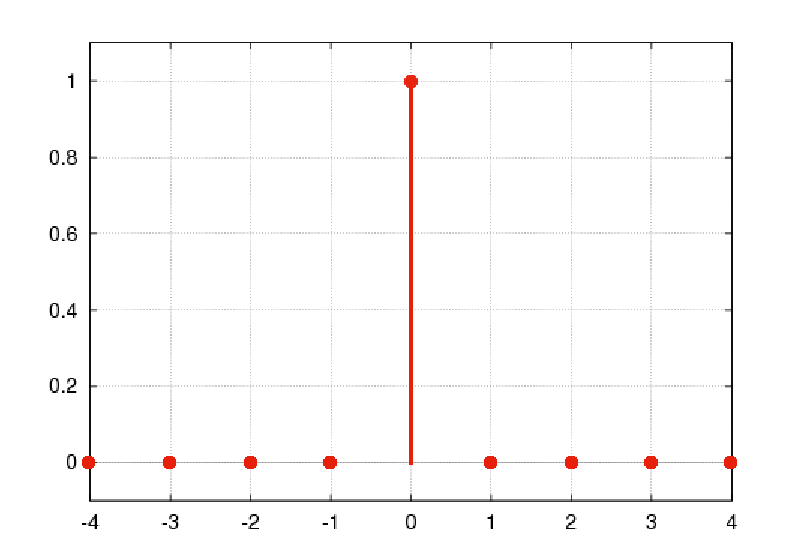
\includegraphics[width=0.5\textwidth]{figs/imp.eps}
      \end{center} }
     \onslide*{3}{
     \begin{center}
        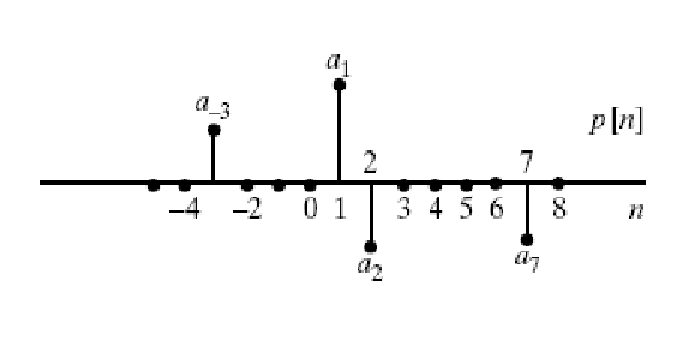
\includegraphics[width=0.5\textwidth]{figs/2_4.eps}
     \end{center} }
     \onslide*{4-11}{
     \begin{center}
        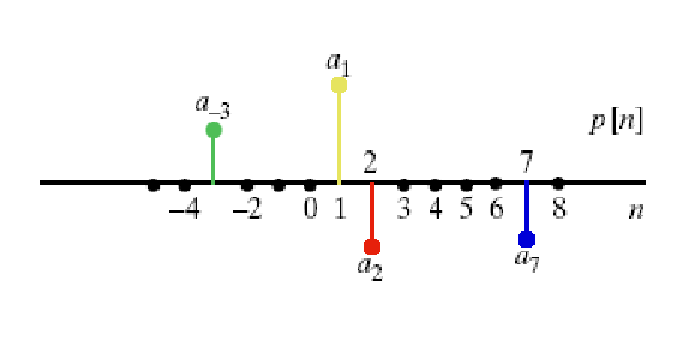
\includegraphics[width=0.5\textwidth]{figs/2_4a.eps}
     \end{center} }
     \onslide*{5}{
     \begin{center}
        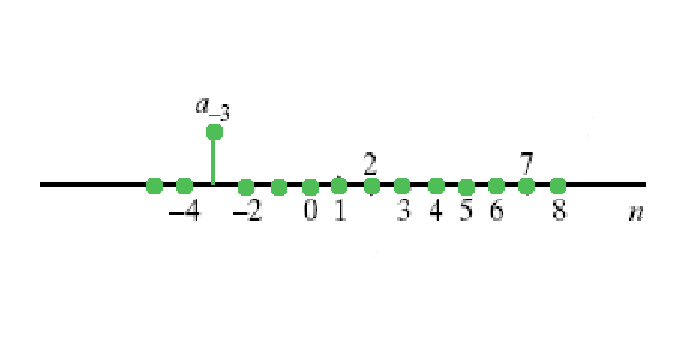
\includegraphics[width=0.5\textwidth]{figs/2_4b.eps}
     \end{center} }
     \onslide*{6}{
     \begin{center}
        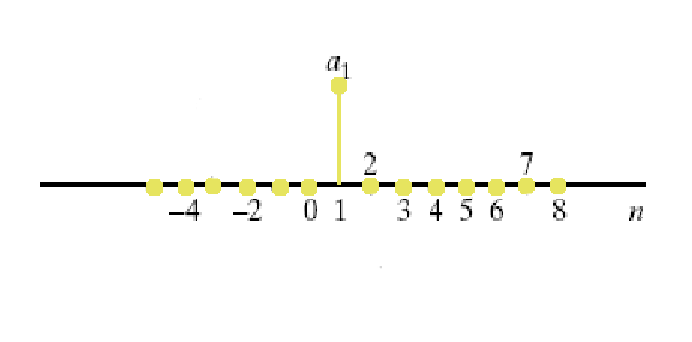
\includegraphics[width=0.5\textwidth]{figs/2_4c.eps}
     \end{center} }
     \onslide*{7}{
     \begin{center}
        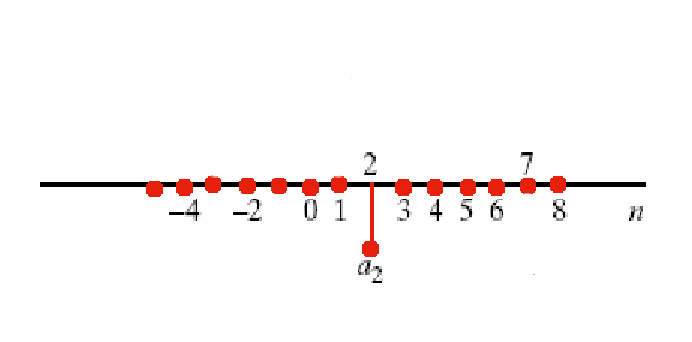
\includegraphics[width=0.5\textwidth]{figs/2_4d.eps}
     \end{center} }
     \onslide*{8}{
     \begin{center}
        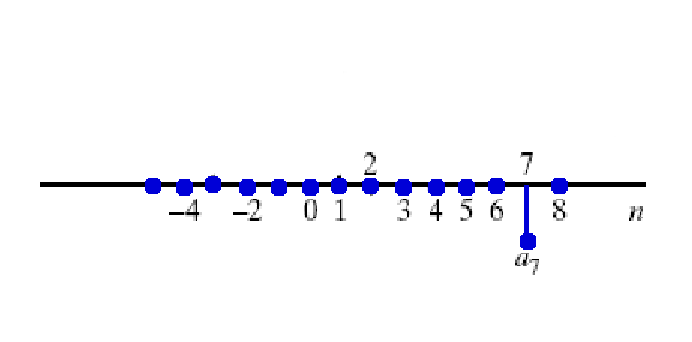
\includegraphics[width=0.5\textwidth]{figs/2_4e.eps}
     \end{center} }
     \onslide*{9}{
     \begin{align*}
        p[n] =& a_{-3}\delta [n+3]+a_{1}\delta [n-1]+\\
              &a_{2}\delta [n-2]+a_{7}\delta [n-7]
     \end{align*}}
     \onslide*{10}{
     \begin{align*}
        p[n] =& p[-3]\delta [n+3]+p[1]\delta [n-1]+\\
              & p[2]\delta [n-2]+p[7]\delta [n-7]
     \end{align*}}
     \onslide*{11}{
     \begin{equation*}
        \boxed{x[n]=\sum_{k=-\infty}^{\infty}x[k]\delta [n-k]}
     \end{equation*}}
    \end{itemize}
\end{slide} 

\begin{slide}[toc=]{Sequências básicas 2}
\begin{itemize}
 \item Degrau unitário:
     \onslide*{1-2}{
     \begin{equation*}
      u[n]=\begin{cases}
                  1, & n \geq 0,\\
                  0, & n < 0,
                 \end{cases}
    \end{equation*}}
   \onslide*{2}{
   \begin{center}
     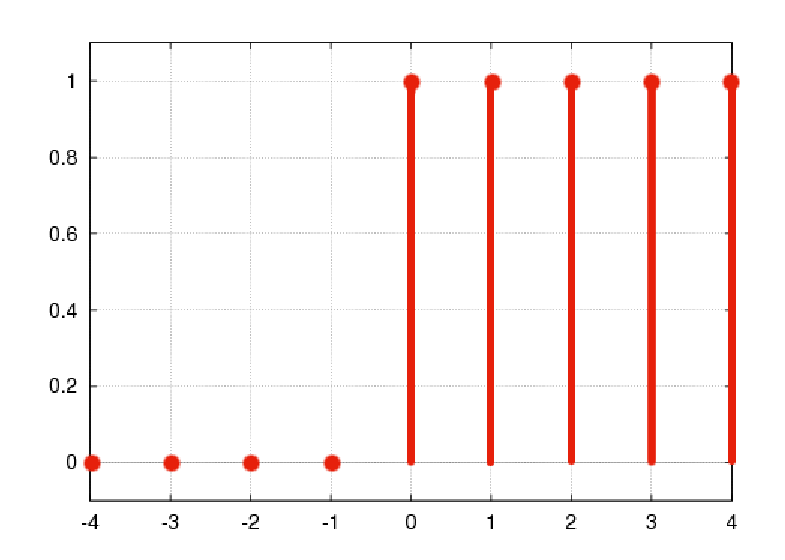
\includegraphics[width=0.5\textwidth]{figs/degrau.eps}
   \end{center} }
   \onslide*{3}{
      \begin{itemize}
         \item Identidades importantes:
         \begin{equation*}
            u[n]=\sum_{k=-\infty}^{n}\delta [k]
         \end{equation*}
         \begin{equation*}
            u[n]=\sum_{k=0}^{\infty}\delta [n-k]
         \end{equation*}
         \begin{equation*}
            \delta [n]=u[n]-u[n-1]
         \end{equation*}
      \end{itemize}
   }
\end{itemize}
\end{slide} 
\end{document}
